\chapter{Applications of the Derivative}
\section{General}\begin{enumerate}

\item  Describe briefly as many applications of derivatives as you can.  Organize these applications in a concept map. 

\item  Determine if each of the following is always true or not always true.  If it is always true, give an argument to support your claim.  If it is not always true, give a counterexample.  
\begin{enumerate}
	\item 	If $f$ is differentiable at $a$, then $$\mathop {\lim }\limits_{x \to a} f(x)$$ exists.
	\item	If $f(c)$ is a local maximum of $f$, then $f'(c) = 0.$
	\item	If $(c, f(c))$ is an inflection point, then $f(c)$ is not a local maximum of $f$.  \cite{MR}
\end{enumerate}

\item  I have a pet polynomial function and I never learned how to share very well so ``You can't have it!''  My mother always says that nobody likes a smart aleck (not her exact words) but you have a chance to be one if you can tell me as much about what my pet function looks like without even knowing what the function is.

\item  If $f'\left( x \right) \le 2$ for all $x$, what is the largest possible increase in the values of $f$ on $[0, 6]$?

\item  Look back at the homework and writing assignments you have done so far and identify concepts that you feel you know the best.  Identify areas that you need to improve on before the exam.  If you could improve on one concept before the exam, what concept would be the most beneficial to you and why? Which are the trickiest?

\item  Write up to 5 distinct questions from the material in this chapter that I might ask on an exam about the following information: Mean Value Theorem.

\item  Write up to 5 distinct questions from the material in this chapter that I might ask on an  about the following information: $f(x) = 3x^3 - 6x$.

\item  Write up to 5 distinct questions from the material in this chapter that I might ask on an exam about the following information:  maxima, minima.

\end{enumerate}\section{Extremes and Optimization}\begin{enumerate}

\item  A friend of yours has missed class (again!) and needs to know how to find absolute extrema.  Gently explain the procedure to her by going through an example.  

\item  Compare the extrema of the 2 functions $f(x)$ and $g(x)$ such that $f(x) - g(x) = 5$ for all $x$. 

\item  Explain the conditions under which a graph is guaranteed to have an absolute maximum and absolute minimum.  Show, using examples, that those conditions are necessary (i.e., if you eliminate one condition, find a graph that does not have the absolute extrema.)

\item  Explain the difference between relative extrema and absolute extrema.  If we consider functions on $(-\infty, \infty)$, are we guaranteed to find relative extrema? If we consider functions on $(-\infty, \infty)$, are we guaranteed to find absolute extrema? If we consider functions on a closed interval, are we guaranteed to find relative extrema? If we consider functions on a closed interval, are we guaranteed to find relative extrema?  Compare and contrast each of these situations.

\item  Find the maximum value of $f(x) = x^3  - 3x$ on the set of real numbers $x$ satisfying $x^4  + 36 \le 13x^2 .$

\item  If $f'(a) < 0 < f'(b)$ and $a < c < b$, is $c$ guaranteed to be a maximum as in the first derivative test?

\item  If $f''(c) > 0$ is c guaranteed to be a minimum as in the second derivative test?

\item  Is it true that a discontinuous function cannot have both an absolute maximum and an absolute minimum value on a closed interval?  \cite{FWG}

\item  It can be said that $$g(x) = \sqrt {f(x)} $$ is minimized by exactly the same $x$-values(s) as $f(x)$ (for $f(x) \ge 0$).  Explain why this is true and for which of the following functions it is also true.
\begin{enumerate} 
	\item $g(x) = \ln \left( {f(x)} \right)$ for $f(x) > 0$	
	\item $g(x) = \left( {f(x)} \right)^2 $	
	\item $g(x) = e^{f(x)} $
	\item $g(x) = \sin \left( {f(x)} \right)$
	\item $g(x) = \left( {f(x)} \right)^3 $
\end{enumerate}

\item  It is important to understand mathematical language and one way to test your knowledge is to ask for specific information in a problems.  In a problem about relative extrema, I could ask for critical numbers, critical values, maximum value, minimum value, or the location of the maximum or minimum.  In each case explain how you know whether to give an $x$-value, a $y$-value, or an ordered pair.

\item  Suppose some friends complain to you that they can't work any of the optimization problems in the book.   When you ask to see their work, they say that they couldn't even get started.  It has been emphasized in class that sketching a picture and defining variables is a good start.  Part of the benefit of this is to help you get started writing something (anything) down.  Do you think this advice helps?  What do you think is the most difficult aspect of these problems?  Give you friends the best advice you can.  \cite{SM}

\item  We have a theorem that says that a continuous function on a closed interval has an absolute maximum and minimum.  But remember that to apply a theorem, the hypotheses have to be checked first.  What happens if we eliminate one of those hypotheses?  Consider a discontinuous function on a closed interval.
\begin{enumerate}
	\item Find such a function with a minimum but no maximum.
	\item Find such a function with a maximum but no minimum.
	\item Find such a function with neither a maximum nor minimum.
	\item Find such a function with both a maximum and minimum.  \cite{SBS}
	\item Discuss your observations.
\end{enumerate}

\item  We have a theorem that says that a continuous function on a closed interval has an absolute maximum and minimum.  But remember that to apply a theorem, the hypotheses have to be checked first.  What happens if we eliminate one of those hypotheses?  Consider a continuous function on an open interval.
\begin{enumerate}
	\item  Find such a function with a minimum but no maximum.
	\item Find such a function with a maximum but no minimum.
	\item Find such a function with neither a maximum nor minimum.
	\item Find such a function with both a maximum and minimum.  \cite{SBS}
	\item Discuss your observations. 
\end{enumerate}

\item  We know how to find the extreme values of a continuous function $f(x)$ by investigating its values at critical points and endpoints..  But what if there are no critical points of endpoints?  What happens then?  Do such functions really exist?  \cite{FWG}

\item  What is the difference between a critical point and a critical number?  Compare and contrast the processes for finding critical numbers in the case of relative extrema on 
$(-\infty, \infty)$ versus absolute extrema on $[a, b]$.  How does this distinction help us eliminate work in application problems?

\item  What is the first-derivative test?  How do you use it?  Why does it work?  What does it tell you?  What do you need to be careful about?\end{enumerate}\section{Rates of Change}\begin{enumerate}

\item  Consider this problem: Find 2 nonnegative numbers so that the sum of the first and twice the other is 12 and the product is a maximum.  In this problem, what is the function you are trying to optimize?  What is the constraint(s)?  Explain these 2 equations, how you use them, their relationship to each other, how you know which is which, etc.

\item  Consider this problem: What is the largest possible area for a right triangle whose hypotenuse is 5 cm long?  In this problem, what is the function you are trying to optimize?  What is the constraint(s)?  Explain these 2 equations, how you use them, their relationship to each other, how you know which is which, etc.

\item  Sam the bartender prepares Norm and Cliff each a Scotch and Water.  The percentage concentration of pure scotch in their drinks is 6.25\%.  Each has an infinitely large glass.

\begin{enumerate}
	\item Before Norm has a chance to start drinking, Vera starts adds water to his drink at a constant rate.  Draw a graph that represents the percentage concentration of pure scotch as a function of the number of ounces of water added by Vera to Norm's drink.  Is this function concave up or down?
	\item Before Cliff has a chance to start drinking Carla calls Cliff a wimp, grabs his drink and adds pure scotch to it at a constant rage.  Draw a graph that represents the percentage concentration of pure scotch as a function of the number of ounces of water added by Vera to Cliff's drink.  Is this function concave up or down? 
\end{enumerate}

\item  Suppose that $f(t)$ represents your elevation after $t$ hours on a mountain hike.  If you stop to rest, explain why $$f'(t) = 0$$ at that point.  Discuss the circumstances under which you would be at a local maximum, local minimum or neither.  \cite{SM}

\item  Two crash test dummies are testing a '72 Pinto station wagon that has been refitted with airbags.  Listen to them, plot their velocity function, and then answer these questions.  What is the domain of the velocity function?  On what interval is Mack and Biff's velocity increasing?	 On what interval is their velocity decreasing?  Is this a continuous function?
\\ {\bf{Mack}}:  Turn the car on, Biff, and let's get going.  We've got an appointment with that brick wall 400 meters ahead.
\\ {\bf{Biff}}:  So, I'm supposed to speed up to 30 m/sec?
\\ {\bf{Mack}}:  Yeah.  When we reach that speed we should be 250 meters down the track.  And then we maintain that speed until we are 50 meters in front of the wall.
\\ {\bf{Biff}}:  And then we slow down so that we hit the wall going 25 m/sec, right?
\\ {\bf{Mack}}:  Riiiiiiggggghhhhhhhhtttttttt!!!!!!!   

\item  What can you say about the rate of change of a constant function?  A linear function?  An exponential function?  A power function?  \cite{SMo}

\item  What is the formula for the volume of a cube?  Its surface area?  What is the formula for the volume of a sphere?  Its surface area?  Find the rate of change of the volume of a cube with respect to the length of one of its edges.  How does this compare to the surface area of the cube?  Find the rate of change of the volume of a sphere?  How does this compare to the surface area of the cube?

\end{enumerate}\section{Mean Value Theorem}\begin{enumerate}

\item  Compare and contrast Rolle's Theorem (RT) and the Mean Value Theorem (MVT).  

\item  Compare and contrast the Intermediate Value Theorem (IVT) and the Mean Value Theorem (MVT).  

\item  Your pesky friend has missed class one more time.  This time he missed the discussion on the Mean Value Theorem (MVT).  After giving him a tactful and gentle lecture on attending class and abusing your friendship, carefully and clearly explain the hypotheses and conclusion of the MVT to him.  Give him some examples of graphs to show what the hypotheses mean.  Using a graph, explain the conclusion of the MVT to him.

\item  Explain how the Mean Value Theorem can be used to prove that, if $f'\left( x \right) = 0$ for all $x$, then $f$ is a constant function.

 \end{enumerate}\section{Graphs and the Derivative}\begin{enumerate}

\item  Apply the second derivative test to $f(x) = x^4$ at the critical number $x = 0$.  Discuss.

\item  If $f'(c) = 0$, is $(c, f(c))$ guaranteed to be an extreme?   Explain and then describe how to determine if $(c, f(c))$ is an extreme?  

\item  Back in the dark ages when I first learned the $x$-coordinate of the vertex of a parabola 
$y = ax^2 + bx + c$ was $$x =  - {b \over {2a}},$$ I didn't know why it worked.  Here you will prove this result is in 2 different ways.

\begin{enumerate}
	\item Assume that a parabola is symmetric.  So the vertex will fall exactly halfway between the $x$-intercepts.  Find the average of the x-intercepts of $y = ax^2 + bx + c$.  
	\item The vertex of a parabola is at the point on the curve where the tangent is horizontal.  Use calculus to find the $x$-coordinate of the vertex.
\end{enumerate}


\item  Can the graph of a function have more inflection points than critical points?  \cite{EP}

\item  Consider the function $f(x) = 5x^2	+ 13x - 6$.  Graph this function on the interval $(-3, 3)$.  Select 5 different values of $x$ from the interval $(-3, 3)$ and place those values in a table in ascending order.  Draw the tangent line to the graph for each value of $x$ you chose.  Find the slope of these tangent lines and enter the slopes in the table.  As you move from left to right on the graph, are the slopes of the tangent lines increasing or decreasing?  What does this say about the derivative of $f'(x)?$    

\item  Consider the function $f(x) = \ln x$ . Graph this function on the interval $(-1, 5)$. Select 5 different values of $x$ from the interval $(-1, 5)$ and place those values in a table in ascending order.  Draw the tangent line to the graph for each value of $x$ you chose.  Find the slope of these tangent lines and enter the slopes in the table.  As you move from left to right on the graph, are the slopes of the tangent lines increasing or decreasing?  What does this say about the derivative of $f'(x)?$

\item  Describe the relationship of the graph of the derivative to the graph of the function. \cite{SBS}

\item  Find constants $A$, $B$, $C$ and $D$ that guarantee that the graph of $$f(x) = 3x^4  + Ax^3  + Bx^2  + Cx + D$$ will have horizontal tangents at $(2, -3)$ and $(0, 7)$.  There is a third horizontal tangent; find it.  Then, for all 3 points, determine whether each corresponds to a relative maximum, a relative minimum, or neither.  \cite{SBS}

\item  Find the critical points of $$f(x) = 2x^3  + 3x^2  - 12x + 11.$$  Apply the first derivative test to $$f(x) = 2x^3  + 3x^2  - 12x + 11$$ to classify these critical points.  Apply the second derivative test to $$f(x) = 2x^3  + 3x^2  - 12x + 11$$ to classify these critical points.  Compare and contrast the application of these 2 tests.  In your writing, consider the application of these tests to more complicated functions.  Are there any functions for which either test fails?

\item  Find the domain of the graph $$f(x) = x^{{2 \mathord{\left/ {\vphantom {2 3}} \right. \kern-\nulldelimiterspace} 3}} \left( {5 - 2x} \right).$$  What does this tell us about the appearance of the graph?  Now graph this function on your calculator.  Is the result consistent with what the graph should look like?  If it is not, find a way to make the calculator do the right thing.  (Remember you are smarter than the calculator.)

\item  For each of the following, try to sketch the function.  If you can sketch it, explain its features and their relationship to the values of the derivatives.  If you cannot sketch it, explain what the contradiction is.\begin{enumerate}
\item A continuous function on $[a, b]$ with a critical point $c$ between $a$ and $b$ but with no extreme value on $(a, b)$.		
\item A differentiable function on $[a, b]$ with a critical point $c$ between $a$ and $b$ but with no extreme value on $(a, b)$.
\item A continuous function on $[a, b]$ with 2 critical points between $a$ and $b$ but with no extreme value on $(a, b)$. 	
\item A continuous function on $[a, b]$ with a local minimum and a local maximum but only one critical point in $(a, b)$.  \cite{EP} \end{enumerate}

\item  For each of the following, try to sketch the function.  If you can sketch it, explain its features and their relationship to the values of the derivatives.  If you cannot sketch it, explain what the contradiction is.
\begin{enumerate}
\item A continuous function on $[a, b]$ with a local minimum and a local maximum and exactly 3 critical points in $(a, b)$.		
\item A continuous function on $[a, b]$ with 3 local maxima but only a single local minimum in $(a, b)$.
\item A function that has 2 distinct critical points that are not separated by an inflection point?  \cite{EP}  \end{enumerate}

\item  For each of the following, try to sketch the function.  If you can sketch it, explain its features and their relationship to the values of the derivatives.  If you cannot sketch it, explain what the contradiction is.
\begin{enumerate}
\item A function which is increasing on $(-\infty, \infty)$ and has a maximum at $x = 2$.		
\item A function that is always negative and always increasing.
\item A function with 2 $x$-intercepts and no minima. 	
\item A function with no $x$-intercepts and no $y$-intercepts. \end{enumerate}

\item  For each of the following, try to sketch the function.  If you can sketch it, explain its features and their relationship to the values of the derivatives.  If you cannot sketch it, explain what the contradiction is.
\begin{enumerate}\item A function with exactly 2 maxima and no minima.	
\item A continuous function with exactly 2 maxima and no minima.
\item A function with no extrema.	
\item A significantly different function with no extrema. \end{enumerate}

\item  For each of the following, try to sketch the function.  If you can sketch it, explain its features and their relationship to the values of the derivatives.  If you cannot sketch it, explain what the contradiction is.
\begin{enumerate}\item A polynomial of odd degree that has neither a local minimum value nor a local maximum value. 	
\item A polynomial function of even degree that has neither an absolute minimum value nor an absolute maximum value.  \cite{EP} \end{enumerate}

\item  For this writing assignment you need to first complete the following experience.  You will work in groups of 3.  
\\ {\bf{Round 1}}:  {\bf{Step 1}}:  Student A sits back-to-back with student B while student C is in a position to watch what is going on.  Student A is given a graph and has to describe that graph to Student B.  Student B will try to reproduce the graph by listening to Student A.  Students B and C cannot talk except that Student B can ask Student A to slow down or to continue.  Student C should monitor the process and keep everyone on task.  
\\ {\bf{Step 2}}: After Student A has described the graph and B has drawn it, compare the graphs.
\\{\bf{Step 3}}:  In your group discuss how the describing/drawing went and make plans for improving the process.
\\{\bf{Rounds 2 and 3}}:  Repeat Round 1 except that each student must assume a new role.  At the end of the 3 rounds each student must have been a describer once, a drawer once, and an observer once.
\\{\bf{To turn in}}: After reviewing the process, how would you recommend as the best way to describe the graph.  Provide details and possibly examples.

\item  If $f'(x)$ does not exist at $x = a$, does that guarantee that $a$ is a critical number for $f$?

\item  If $f''(c) = 0,$ is $c$ guaranteed to be an inflection point?  If $f''(c) \ne 0,$ is it guaranteed that  $c$ is not an inflection point?

\item  If a statement is false, give a counterexample.  If a statement is true, explain why. \begin{enumerate}
\item If $f$ is concave up, then $-f$ is concave down.
\item If $f$ is concave up and $g$ is concave up, then $fg$ is concave up.
\item If $f$ is concave up and $g$ is concave down, then $fg$ is neither concave up nor down. \end{enumerate}

\item  If I ask you to match graphs of derivatives to graphs of functions, what do you look for?

\item  On what intervals is $f$ increasing and decreasing if $${{df} \over {dx}} = 6\left( {x - 1} \right)\left( {x - 2} \right)^2 \left( {x - 3} \right)^3 \left( {x - 4} \right)^4 .$$  What are the extrema of $f$?  \cite{FWG}

\item  Prove or disprove:  If the graphs of $f$ and $g$ are both concave up on an interval, then the graph of their sum $f + g$ is also concave up on that interval.  \cite{SBS}

\item  Sketch a curve for which $f(x) < 0$, $f'(x)< 0$, and $f'(x)$ is decreasing on $(-\infty, \infty)$.

\item  In the following graph one of the curves is $f(x)$ and the other curve is its derivative.  Which is which?  Explain your answer. 
%put Chapter4Fig.jpg here

\item  Let $$f(x) = \root 5 \of {x^3  - Lx + 1} $$ where $L$ is the number of letters in your last name.  Let $g(x)$ be another function such that the tangent line to $g(x)$ at $x = 2$ is $y = 7x - 4S$, where $S$ is the number of sisters you have.  For which of the following functions can we determine the tangent line from the above information?  If it is possible to determine it, do so.  If there is not enough information to determine it, explain why not. \cite{FWG}
\begin{enumerate}
	\item $A(x) = f(x) + g(x)$ at $x = 2$ 
	\item $B(x) = f(x) g(x)$ at $x = 2$
	\item $C(x) = f(x)/g(x)$ at $x = 2$ 
	\item $D(x) = f(g(x))$ at $x = 2$
	\item $E(x) = g(f(x))$ at $x = 2$
\end{enumerate}

\item  Let $$f(x) = x^4  + x^3  - 8x^2  - 12x.$$  Find the first and second derviatives of $f(x)$.  Discuss whether each of the following statements is true or false. \begin{enumerate}
\item $f$ is increasing at $x = 1$.
\item $f$ has a relative minimum at $x = -2$.
\item $f$ is concave down at $x = 1$.
\item $f$ has a root at $x = 1$.  \cite{SMo}\end{enumerate} 

\item  Suppose that you have a differentiable function $f(x)$ with 2 critical numbers.  You computer has shown you a graph that looks like Figure \ref{Chapter4Figureb}.  Is it possible that there are any important points not shown in the window you used to display this graph?  Would your answer change if the function had 3 critical numbers?  \cite{SM}

%put Chapter4Figb.jpg here

\begin{figure}[ht]
	\centering
		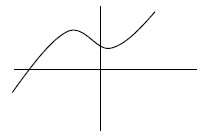
\includegraphics{TeXGraphics/Chapter4Figb.jpg}
	\caption{A function}
	\label{Chapter4Figureb}
\end{figure}

\item  The goal of investing in the stock market is to buy low and sell high.  But, how can you tell whether a price has peaked or not?  Once a stock price goes down, you can see that it was at a peak but then it is to late to do anything about it!  Concavity can help.  Suppose a stock price is increasing and the price curve is concave up.  Why would you suspect that it will continue to rise?  Is this a good time to buy?  Now, suppose the price is increasing but the curve is concave down.  Should you be preparing to sell?  Buy?  Finally, suppose the price is decreasing.  If the curve is concave up, should you buy or sell?  What if the curve is concave down?  \cite{SM}

\item  The upcoming exam will require you to understand graphing and will have some pretty involved multi-step problems.  First, complete this problem:  ``Consider the function $$f(x) = \root 3 \of x \left( {27 - x} \right).$$  Graph this function by first listing all key features.  Pay attention to how easy or difficult each part of this problem is.  Did you remember all the key features?  If you could improve one part of these problems, what area would be the most beneficial to you and why?  What parts are the easiest for you?  Which are the trickiest?

\item  What is the relationship between $x$-intercepts and the intervals where a function is positive and negative?  What is the relationship between extrema and the intervals where a function is increasing and decreasing?  What is the relationship between inflection points and the intervals where a function is concave up and down?

\item  What is the second-derivative test?  How do you use it?  Why does it work?  What does it tell you?  What do you need to be careful about?

\item  Compare and contrast the graphs of polynomial and rational functions.

\item  Graph $$f(x) = \left| x \right|$$ on the interval [-1, 2].  What is the sign of $$f'\left( x \right)$$ on (-1, 0)?  What is the sign of $$f'\left( x \right)$$ on (0, 2)?  Can we apply the First Derivative Test to $f(x)$ on [-1, 2]?

\item  Fill in the blank and then explain your choices:  Every $\mathop {\underline {\quad \quad \quad \quad \quad } }\limits_{{\rm{global}}\ \  {\rm{or}}\ \   {\rm{local}}} $
 maximum of the function $f$ is also a $\mathop {\underline {\quad \quad \quad \quad \quad } }\limits_{{\rm{global}}\ \  {\rm{or}}\ \  {\rm{local}}} $
 maximum of $f$.

\item  Consider a polynomial function $P(x)$ of degree $n$.  What is the maximum number of $x$-intercepts $P$ could have?  The maximum number of critical points?  The maximum number of inflection points?  Is it possible for a polynomial to attain the maximum number of inflection points but only have 1 critical point (possible of a high multiplicity)? 

\end{enumerate}\section{Asymptotes}\begin{enumerate}

\item  Compare and contrast horizontal and vertical asymptotes.  Include both analytical and visual examples to illustrate the points you make.  Discuss the examples numerically.

\item  Explain why polynomials never have  vertical or horizontal asymptotes.  \cite{SM}

\item  Find constants a and b that guarantee that the graph of the function defined by $$f(x) = {{ax + 5} \over {3 - bx}}$$ will have a vertical asymptote at $x = 5$ and a horizontal asymptote at 
$y = -3$. \cite{SBS}  In general, discuss how the values of $a$, $b$, $c$ and $d$ determine the horizontal and vertical asymptotes of $$f(x) = {{ax + d} \over {bx + c}}.$$

\item  Find the horizontal and vertical asymptotes of a variety of rational functions.  Make conjectures that would help you find these asymptotes without all the fuss.

\item  If $x = 2$ is a vertical asymptote of the graph of the function $y = f(x)$, describe what happens to the $x$- and $y$-coordinates of a point moving along the graph, as $x$ approaches 2.

\item  There are other types of asymptotes than just vertical and horizontal.  Before looking at slant and polynomial asymptotes, let's first look at a new way to look at vertical asymptotes.  Find the (right) horizontal asymptote $y = a$ of $$f(x) = {{2x} \over {3x + 1}}.$$  Now calculate the limit $$\mathop {\lim }\limits_{x \to \infty } \left[ {f(x) - a} \right].$$  Try this for several other rational functions.  Look at the graphs of $f(x)$ and $y = a$ and describe their relationship for large values of $x$.
	\\\mbox{}$\ \ \ \ \ $Find a linear function $l(x) = ax + b$ such that $$\mathop {\lim }\limits_{x \to \infty } \left[ {f(x) - l(x)} \right] = 0$$ for the function $$f(x) = {{x^3  + 2x^2  - 1} \over {x^2  - 1}}.$$  Graph $f(x)$ and $l(x)$ and describe their relationship for large values of $x$.  The line $l(x)$ is called a slant asymptote.  Make a general description of rational functions that have slant asymptotes.
	\\\mbox{}$\ \ \ \ \ $For each of these functions, find a polynomial $P(x)$ such that $$\mathop {\lim }\limits_{x \to \infty } \left[ {f(x) - P(x)} \right] = 0.$$




\begin{enumerate}
\item $f(x) = {{x^4 } \over {x + 1}}$
\item $f(x) = {{x^5  - 1} \over {x + 1}}$
\item $f(x) = {{x^6  - 2} \over {x + 1}}\ \ \cite{SM}$  
\end{enumerate}
Graph each $f(x)$ and $P(x)$ and describe their relationship for large values of $x$.  These polynomials are called polynomial asymptotes.  Make a general description of rational functions that have polynomial asymptotes.

\item  While studying for an exam, a friend says that a graph is not allowed to touch an asymptote.  What do you think?

\item  Investigate the validity of this statement: When finding horizontal asymptotes you only have to calculate $$\mathop {\lim }\limits_{x \to \infty } f(x)$$ because $$\mathop {\lim }\limits_{x \to  - \infty } f(x)$$ is always the same thing. 

\item  Investigate the validity of this statement:  Every rational function has vertical asymptotes.

\item  Investigate the validity of this statement:  A graph cannot have both a vertical asymptote and a slant asymptote.

\end{enumerate}\section{L'Hospital's Rule and Indeterminate Forms}

\begin{enumerate}

\item  Explain in your own words why $0^\infty  $ and $0^{ - \infty } $ are not indeterminate forms.  \cite{EP}  Be sure to explain what an indeterminate form is and why these two forms do not fit in that category.  As always, examples where these 2 forms occur would be useful.

\item  How do you use L'Hospital's Rule?  When can you apply it?  What does it help us do?  What happens if you apply it at times when you shouldn't?  Using a picture, give an overview of why L'Hospital's Rule works.

\item  What is an indeterminate form?  Give examples of indeterminate forms and of forms that are not indeterminate.  What distinguishes these 2 forms?  Give examples to illustrate what makes an indeterminate form indeterminate.

\item  A friend of yours has this work on their paper.  
		$$\begin{array}{rcl} \displaystyle{\mathop {\lim }\limits_{x \to 0} {{1 - \cos x} \over {\sec x}} }&\mathop  {=} \limits^H 
&  \displaystyle{\mathop {\lim }\limits_{x \to 0} {{\sin x} \over {\sec x\tan x}} }\cr \mbox{}&&\cr   
		&=& \displaystyle{\mathop {\lim }\limits_{x \to 0} {{\sin x} \over {\sec x\tan x}}} \cr \mbox{}&&\cr   
		&=& \displaystyle{\mathop {\lim }\limits_{x \to 0} {{\cos x} \over {\sec x}} }\cr     \mbox{}&&\cr   
		&= &\displaystyle{{1 \over 1}} \cr  \mbox{}&&\cr   
		&=&1\end{array} $$
Show them with the graph of $$f(x) = {{1 - \cos x} \over {\sec x}}$$ that they probably got the wrong limit.  Help them understand the problems in their calculations.

\item Consider the following calculation of  $\displaystyle
\mathop {\lim }\limits_{x \to \infty } \left( {1 + {\textstyle{2 \over x}}} \right)^x 
$.  Explain what has been done in each step of the calculation and why.

$$
\begin{array}{rcl}
  L 
  	&= 
  		&\mathop {\lim }\limits_{x \to \infty } \left( {1 + {2 \over x}} \right)^x  \cr 
  		\ln L
  	& =
  		& \mathop {\lim }\limits_{x \to \infty } \ln \left( {1 + {2 \over x}} \right)^x  \cr 
   	&=
   		& \mathop {\lim }\limits_{x \to \infty } x\ln \left( {1 + {2 \over x}} \right) \cr 
   	&=
   		& \mathop {\lim }\limits_{x \to \infty } {{\ln \left( {1 + {2 \over x}} \right)} \over {e{1 \over x}}} \cr 
  	&\mathop  = \limits^H &\mathop {\lim }\limits_{x \to \infty } {{{1 \over {1 + {2 \over x}}} \cdot \left( { - {2 \over {x^2 }}} \right)} \over { - {1 \over {x^2 }}}} \cr 
  	& =
  		& \mathop {\lim }\limits_{x \to \infty } {2 \over {1 + {2 \over x}}} \cr 
  	& =
  		& 2 \cr 
  \ln L 
  	&= 
  		&2 \cr 
  L
  	& =
  		& e^2  \cr 
  		\end{array}
$$


\item  Compute $$\mathop {\lim }\limits_{x \to 0^ +  } x^x $$ graphically, numerically, and analytically.  Compare, contrast and reconcile these three methods.  \cite{SBS}


\item  Let 
$$f(x) = \left\{ \begin{array}{lcr}  x + 2, 
     &\ \ \mbox{}& x \ne 0 \cr   
     0, & &x = 0 \cr \end{array}  \right.$$ 
and 
$$g(x) = \left\{ \begin{array}{lcr}  x + 1, 
     &\ \ \mbox{}& x \ne 0 \cr   
     0, & & x = 0 \cr \end{array} \right. .$$  
Show that $$\mathop {\lim }\limits_{x \to 0} {{f'(x)} \over {g'(x)}} = 1$$ and $$\mathop {\lim }\limits_{x \to 0} {{f(x)} \over {g(x)}} = 2.$$  
Why does this not contradict L'Hospital's Rule?  \cite{FWG}


\item  L'Hospital's Rule is not some magic tonic that will work for any limit.  Discuss the issues with the following limits in regard to L'Hospital's Rule.
\begin{enumerate}\item $\mathop {\lim }\limits_{x \to 1} {{x - 1} \over {\left| {x - 1} \right|}}$ \item $\mathop {\lim }\limits_{x \to \infty } {x \over {\sqrt {x^2  - 1} }}$ \item $\mathop {\lim }\limits_{x \to 0} {{1 - \cos x} \over {x^2 }}$ \item $\mathop {\lim }\limits_{x \to 1} {{x^{10}  + 1} \over {x - 1}}$\end{enumerate}

\item  L'Hospital's Rule states that, in certain situations, the ratios of function values approaches the same limit as the ratios of corresponding derivatives (rates of change).  Graphically, this may be hard to understand.  The get a handle on this, consider $${{f(x)} \over {g(x)}}$$ where both 
$f(x) = ax + b$ and $g(x) = cx + d$ are both linear functions.  Explain why the value of $$\mathop {\lim }\limits_{x \to \infty } {{f(x)} \over {g(x)}}$$ should be the same as $$\mathop {\lim }\limits_{x \to \infty } {{f'(x)} \over {g'(x)}}.\ \cite{SM}$$ 

\item  List as many indeterminate forms as possible.  Why are these forms called indeterminate?  For which of these forms can we use L'Hospital's Rule directly?  How would you transform the other indeterminate forms into ones that we can use L'Hospital's Rule?

\item  When we try to evaluate a limit and find a form such as $${\infty  \over \infty }$$ this is called indeterminate because there exist limits of this form for which the result is any real number.  Explain how to find examples of differentiable functions $f$ and $g$ such that $$\mathop {\lim }\limits_{x \to \infty } f(x) = \infty $$ and $$\mathop {\lim }\limits_{x \to \infty } g(x) = \infty $$ such that the limits have the values listed below.
\begin{enumerate}\item	$\mathop {\lim }\limits_{x \to \infty } {{f(x)} \over {g(x)}} = 3$\item		$\mathop {\lim }\limits_{x \to \infty } {{f(x)} \over {g(x)}} = 0$\item		$\mathop {\lim }\limits_{x \to \infty } {{f(x)} \over {g(x)}} = \infty $  \cite{FWG}\end{enumerate}

\item  You and a friend decide to compare homework and you find the following results.
\begin{center}{Your friend's paper}\end{center}
	$$\begin{array}{rcl}  \displaystyle{\mathop {\lim }\limits_{x \to 3} {{x - 3} \over {x^2  - 3}}}& = &\displaystyle{\mathop {\lim }\limits_{x \to 3} {1 \over {2x}}} \cr  \mbox{}&&\cr  &= &{1 \over 6} \cr \end{array}$$

\begin{center}Your paper\end{center}
$$\begin{array}{rcl}  \displaystyle{\mathop {\lim }\limits_{x \to 3} {{x - 3} \over {x^2  - 3}}} &=& \displaystyle{{0 \over 6}} \cr   \mbox{}&&\cr  &=& 0 \cr\end{array} $$
Who is right?  \cite{FWG}

\item  Your favorite friend (the one that misses class all the time) has asked you to explain how to find $$\mathop {\lim }\limits_{x \to 0} x^{\sin x} .$$  You decide it would be a good review for you to kindly show him the steps and explain them along the way.

\item  Consider the following limit:  $$\mathop {\lim }\limits_{x \to \infty } x\ln \left( {{{x - 1} \over {x + 1}}} \right) = \infty  \cdot 0 = 0.$$  Using a table, investigate whether this limit was calculated correctly.  Observations?

\item  Consider the following limit:  $$\mathop {\lim }\limits_{x \to \infty } \sqrt {x^2  + 3x}  - x = \infty  - \infty  = 0.$$  Using a table, investigate whether this limit was calculated correctly.  Observations?

\item  Consider the following limit:  $$\mathop {\lim }\limits_{x \to 0^ +  } x^{\tan x}  = 0^0  = 0.$$  Using a table, investigate whether this limit was calculated correctly.  Observations?

\item  The graphs of differentiable functions $f$ and $g$ are shown in Figure \ref{Chapter4Figurec}.  Which of the following is true about $$\mathop {\lim }\limits_{x \to 0} {{f(x)} \over {g(x)}}?$$ \begin{enumerate}\item The limit is less than 0.  \item   The limit is 0.  
\item The limit is 1. \item The limit is greater than 1.  \item The limit does not exist. \end{enumerate}
Explain your solution.  Create another figure similar to Figure \ref{Chapter4Figurec} that would use the same reasoning but would arrive at another answer on the list.  Explain the solution.

%put Chapter4Figc.jpg here
\begin{figure}[ht]
	\centering
		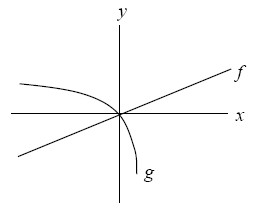
\includegraphics{TeXGraphics/Chapter4Figc.jpg}
	\caption{Two functions}
	\label{Chapter4Figurec}
\end{figure}

\item Provide an annotated calculation of $$
\mathop {\lim }\limits_{x \to 1} x^{{1 \mathord{\left/
 {\vphantom {1 {(1 - x)}}} \right.
 \kern-\nulldelimiterspace} {(1 - x)}}} .
$$


\end{enumerate}


